\documentclass[presentation]{beamer}

\usepackage{appendixnumberbeamer}
\usepackage{amsmath}
\date{14th February 2017}
\usetheme{firedrake}

\newcommand{\KSP}[2]{\ensuremath{\mathcal{K}\left(#1, \mathbb{#2}\right)}}
\newcommand{\ksp}[1]{\KSP{#1}{#1}}

\newcommand{\highlight}[1]{\colorbox{red!20}{\color{black} #1}}

\author{Lawrence Mitchell\inst{1} \and Rob Kirby\inst{2}}
\institute{
\inst{1}Departments of Computing and Mathematics, Imperial College
London
\and
\inst{2}Department of Mathematics, Baylor University
}

\graphicspath{{./\jobname.figures/}}

\newcommand{\arxivlink}[2]{%
  \href{http://www.arxiv.org/abs/#1}%
  {{\small\texttt{arXiv:\,#1\,[#2]}}}%
}
\newcommand{\doilink}[1]{%
  \href{http://dx.doi.org/#1}%
  {{\small\texttt{doi:\,#1}{}}}%
}
\usepackage[url=false,
            doi=true,
            isbn=false,
            style=authoryear,
            firstinits=true,
            uniquename=init,
            backend=biber]{biblatex}

\setbeamertemplate{bibliography item}{}
\renewcommand{\bibfont}{\footnotesize}
\addbibresource{../literature.bib}

\newcommand{\inner}[1]{\left\langle #1 \right \rangle}
\setlength{\bibitemsep}{1ex}
\setlength{\fboxsep}{1pt}

\renewbibmacro{in:}{}
\DeclareFieldFormat[article]{volume}{\textbf{#1}}
\DeclareFieldFormat{doi}{%
  doi\addcolon%
  {\scriptsize\ifhyperref{\href{http://dx.doi.org/#1}{\nolinkurl{#1}}}
    {\nolinkurl{#1}}}}
\AtEveryBibitem{%
\clearfield{pages}%
\clearfield{issue}%
\clearfield{number}%
}

\usepackage{minted}

\title{Programming your (implicit) solver}

\begin{document}

\bgroup
\setbeamertemplate{background}{}
\begin{frame}[standout]

\only<1>{\hspace*{-2em}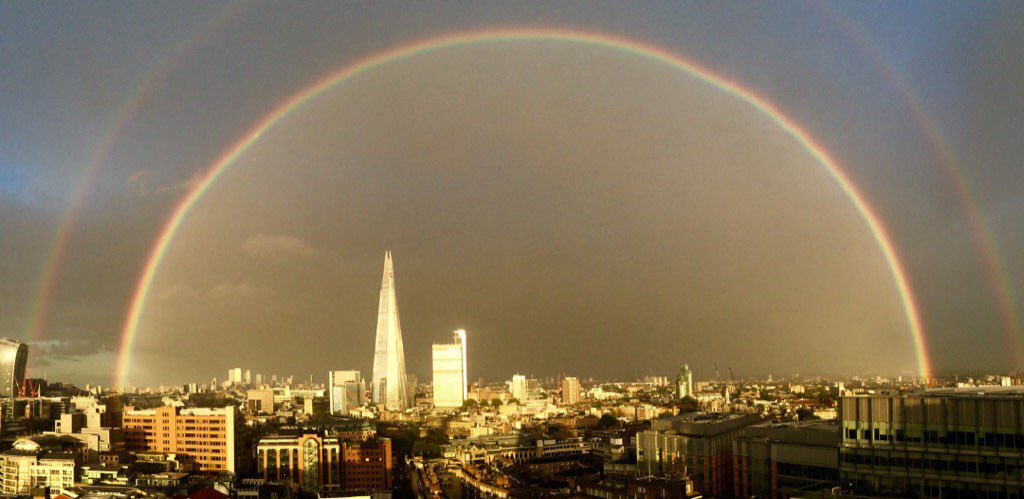
\includegraphics[width=\paperwidth]{rainbow-city}}

\only<2>{\url{http://www.climate-lab-book.ac.uk/2014/end-of-the-rainbow/}}

\begin{center}
  \begin{onlyenv}<2>
    \begin{tikzpicture}
      \node (A) {
\includegraphics[width=\textwidth]{rainbow}};

      \draw[line width=4pt, color=red] (A.south west) -- (A.north
      east);
    \end{tikzpicture}
  \end{onlyenv}
\end{center}
\end{frame}
\egroup

\maketitle

\begin{frame}[fragile]
  \frametitle{Software libraries simplify writing models}
  \begin{columns}
    \begin{column}{0.48\framewidth}
      \begin{block}{Stationary Rayleigh-B\'enard convection}
        \begin{equation*}
          \begin{split}
            -\Delta u + u\cdot\nabla u + \nabla p +
            \frac{\text{Ra}}{\text{Pr}} \hat{g}T &= 0 \\
            \nabla \cdot u &= 0 \\
            - \frac{1}{\text{Pr}} \Delta T + u\cdot \nabla T &= 0
          \end{split}
        \end{equation*}
      \end{block}
    \end{column}
    \begin{column}{0.52\framewidth}
\begin{minted}[fontsize=\tiny,mathescape]{python}
from firedrake import *
mesh = Mesh(...)
V = VectorFunctionSpace(mesh, "CG", 2)
W = FunctionSpace(mesh, "CG", 1)
Q = FunctionSpace(mesh, "CG", 1)
Z = V * W * Q
upT = Function(Z)
u, p, T = split(upT)
v, q, S = TestFunctions(Z)
bcs = [...] # no-flow + temp gradient
nullspace = MixedVectorSpaceBasis(
   Z, [Z.sub(0), VectorSpaceBasis(constant=True), Z.sub(2)])

F = (inner(grad(u), grad(v))
     + inner(dot(grad(u), u), v)
     - inner(p, div(v))
     + (Ra/Pr)*inner(T*g, v)
     + inner(div(u), q)
     + inner(dot(grad(T), u), S)
     + (1/Pr) * inner(grad(T), grad(S)))*dx

solve(F == 0, upT, bcs=bcs, nullspace=nullspace)
\end{minted}
    \end{column}
  \end{columns}
\end{frame}
\begin{frame}
  \frametitle{What about the solver?}
  \begin{itemize}
  \item Such coupled problems are (typically) not amenable to black box solution
    methods.
  \item Direct factorisations reasonable for small problems.
  \item Large problems needs scalable solution, typically block
    factorisations.
  \item Gives many knobs to tweak, may require problem-specific
    auxiliary operators.
  \item How do we capture the abstraction such that automated model
    manipulation is still possible? (e.g.~automated adjoints).
  \end{itemize}
\end{frame}
\begin{frame}
  \frametitle{Block preconditioning}
  Most state of the art preconditioning for multi-variable
  problems is based on block LU factorisations.

  \begin{equation*}
    T = \begin{bmatrix}
      A & 0 \\
      0 & C A^{-1} B^T
    \end{bmatrix}^{-1}
    \begin{bmatrix}
      A & B^T \\
      C & D = 0
    \end{bmatrix}
  \end{equation*}
  has minimal polynomial $T(T - I)(T^2 - T - I) =
  0$ \parencite{Murphy:2000}.

  See \textcite{Ipsen:2001} for the case $D \ne 0$.
\end{frame}

\begin{frame}
  \frametitle{What does this mean}
  \begin{itemize}
  \item Only need inverses of diagonal blocks (and [dense] Schur complements).
  \item Only need the \emph{action} of off-diagonal blocks.
  \item The most efficient (time to solution) strategy is problem and
    parameter dependent:
    \begin{itemize}
    \item Do I invert the blocks well or not?
    \item How many couping terms should I drop?
    \end{itemize}
  \item Need to be able to \emph{configure} the solver without
    changing the code (e.g.~eliminating first row or second?)
  \item Need to treat nested problems.
  \end{itemize}
\end{frame}

\begin{frame}
  \frametitle{Back to Rayleigh-B\'enard}
  Newton needs a linearisation:
  \begin{equation*}
    J = \begin{bmatrix}
      F   & B^T & M_1 \\
      C   & 0   & 0   \\
      M_2 & 0   & K
    \end{bmatrix}.
  \end{equation*}
  \begin{itemize}
  \item Navier-Stokes (top left)
  \item Convection-diffusion for temperature (bottom right)
  \item Coupling in $M_1$ and $M_2$ (non-symmetric).
  \end{itemize}
\end{frame}

\begin{frame}
  \frametitle{Preconditioning}
  Write
  \begin{equation*}
    N = \begin{bmatrix}
      F & B^T\\
      C & 0 \\
    \end{bmatrix} \quad
    \tilde{M}_1 =
    \begin{bmatrix}
      M_1 \\
      0
    \end{bmatrix} \quad
    \tilde{M}_2 = \begin{bmatrix}
      M_2 & 0
    \end{bmatrix}
  \end{equation*}
  and eliminate the Navier-Stokes block, giving system for temperature:
  \begin{equation*}
    S_T = K - \tilde{M}_2 N^{-1} \tilde{M}_1.
  \end{equation*}
  \textcite{Howle:2012} show that $K^{-1}$ is a good preconditioner for
  $S_T$.
\end{frame}
\begin{frame}
  \frametitle{Newton update}
  Solve for the update
  \begin{equation*}
    \delta x = J^{-1} r.
  \end{equation*}

  Write $\mathcal{K}(A, \mathbb{A})$ to denote approximating $A^{-1}$
  using an iteration $\mathcal{K}$ on $A$ using $\mathbb{A}$ as a
  preconditioner.  Then the iteration
  \begin{equation*}
    \KSP{J}{\begin{bmatrix}
      \ksp{N} & 0 \\
      0 & I
    \end{bmatrix}
    \begin{bmatrix}
      I & -\tilde{M}_1 \\
      0 & I
    \end{bmatrix}
    \begin{bmatrix}
      I & 0\\
      0 & \ksp{K}
    \end{bmatrix}}
  \end{equation*}
  empirically converges swiftly, and
  requires only preconditioners $\mathbb{N}$ for Navier-Stokes and
  $\mathbb{K}$ for convection-diffusion.
\end{frame}

\begin{frame}
  \frametitle{Navier-Stokes block \parencite{Elman:2014}}
  A lower Schur complement factorisation of $N$ is a good option.
  Requires $\ksp{F}$ and $\KSP{S_p}{S}$ where $S_p = -C F^{-1} B^T$.

  One option is the \emph{pressure convection-diffusion}
  approximation:
  \begin{equation*}
    \mathbb{S} = \KSP{L_p}{L} F_p \KSP{M_p}{M},
  \end{equation*}
  giving
  \begin{equation*}
    \mathbb{N} = \begin{bmatrix}
      F & 0 \\
      0 & \mathcal{K}(S_p, \KSP{L_p}{L}\,F_p \, \KSP{M_p}{M})
    \end{bmatrix}
    \begin{bmatrix}
      I & 0\\
      -C & I
    \end{bmatrix}
    \begin{bmatrix}
      \ksp{F} & 0 \\
      0 & I
    \end{bmatrix}.
  \end{equation*}

\end{frame}

\begin{frame}
  \frametitle{Things to note}

  \begin{itemize}
  \item We only ever need inverses of diagonal blocks.
  \item Can save memory by applying operators matrix-free.
  \item The inverses are nested, we need ways of controlling the inner
    iterations.
  \item PCD drives an axe through the horizontal split between
    the PDE library and the solver library.
  \end{itemize}

  \begin{block}{PCD}
    Needs the auxiliary discretised operator $F_p$ and approximate
    inverses of the auxiliary operators $L_p$ and $M_p$.
  \end{block}
\end{frame}

\begin{frame}[fragile]
  \frametitle{Firedrake \& PETSc to the rescue}
  PETSc already provides a highly runtime-configurable library for
  \emph{algebraically} composing solvers \parencite{Brown:2012}.

  Firedrake makes it straightforward to build any auxiliary
  operators.

  \begin{block}{A new matrix type}
    We create a new PETSc matrix type in Firedrake that remembers the
    symbolic Jacobian it comes from, and implements matrix-free
    actions.
  \end{block}
  \begin{block}{Firedrake-aware preconditioners}
    Algebraic preconditioners cannot work on shell matrices, so we
    create custom preconditioners that can inspect the symbolic
    information and do the appropriate thing.
  \end{block}
\end{frame}

\begin{frame}[fragile]
  \frametitle{PCD}

\begin{minted}[fontsize=\tiny,mathescape]{python}
class PCDPC(PCBase):
    def initialize(self, pc):
        _, P = pc.getOperators()
        ctx = P.getContext()
        appctx = ctx.appctx
        p, q = ctx.arguments()
        M_p = assemble(p*q*dx)
        L_p = assemble(inner(grad(p), grad(q))*dx
        M_ksp = KSP().create()
        M_ksp.setOperators(M_p)
        L_ksp = KSP().create()
        L_ksp.setOperators(L_p)
        [...] # Some boilerplate elided
        u0 = split(appctx["state"])[appctx["velocity_space"]]
        F_p = assemble(inner(grad(p), grad(q))*dx + inner(u0, grad(p))*q*dx)

    def apply(self, pc, x, y):
        # $y \leftarrow \KSP{L_p}{L} F_p \KSP{M_p}{M} x$
        a, b = self.workspace
        self.M_ksp.solve(x, a)
        self.F_p.mult(a, b)
        self.L_ksp.solve(b, y)
\end{minted}
\end{frame}

\begin{frame}
  \frametitle{How to configure things}

  PETSc provides a ``programming language'' for configuring objects at
  runtime.  It has two operations

  \begin{enumerate}
  \item Value assignment
  \item String concatenation
  \end{enumerate}

  Every object has an \emph{options prefix} which controls where in
  the options database it looks for configuration values.

  This is verbose, but a very powerful idea.  We can control the types
  of individual solves by ensuring that they have different prefixes.
\end{frame}

\begin{frame}[fragile]
  \frametitle{The elided boilerplate}
\begin{minted}[fontsize=\small]{python}
class PCDPC(PCBase):
    def initialize(self, pc):
        ...
        prefix = pc.getOptionsPrefix()
        M_ksp.setOptionsPrefix(prefix + "pcd_Mp_")
        M_ksp.setFromOptions()
        L_ksp.setOptionsPrefix(prefix + "pcd_Lp_")
        L_ksp.setFromOptions()
\end{minted}
\end{frame}

\begin{frame}
  \frametitle{Back to the main event}
  We are solving
  \begin{equation*}
    \KSP{\begin{bmatrix}
        F & B^T & M_1\\
        C & 0 & 0 \\
        M_2 & 0 & K
      \end{bmatrix}}{J}
  \end{equation*}
  using
  \begin{equation*}
    \mathbb{J} =
    \begin{bmatrix}
      \KSP{\begin{bmatrix}
          F & B^T\\
          C & 0
        \end{bmatrix}}{N} & 0\\
      0 & I
    \end{bmatrix}
    \begin{bmatrix}
      I & 0 & -M_1\\
      0 & I & 0 \\
      0 & 0 & I
    \end{bmatrix}
    \begin{bmatrix}
      I & 0 & 0\\
      0 & I & 0\\
      0 & 0 &\ksp{K}
    \end{bmatrix}
  \end{equation*}
  with
  \begin{equation*}
    \mathbb{N} = \begin{bmatrix}
      F & 0 \\
      0 & \mathcal{K}(S_p, \KSP{L_p}{L}\,F_p \, \KSP{M_p}{M})
    \end{bmatrix}
    \begin{bmatrix}
      I & 0\\
      -C & I
    \end{bmatrix}
    \begin{bmatrix}
      \ksp{F} & 0 \\
      0 & I
    \end{bmatrix}
  \end{equation*}
  and
  \begin{equation*}
    S_p = -C \ksp{F} B^T.
  \end{equation*}
\end{frame}

\begin{frame}[fragile]
  \frametitle{First, the temperature solve}
  \small
  \begin{onlyenv}<1>
    \begin{equation*}
      \KSP{J}{%
      \begin{bmatrix}
        \KSP{\begin{bmatrix}
            F & B^T\\
            C & 0
          \end{bmatrix}}{N} & 0\\
        0 & I
      \end{bmatrix}
      \begin{bmatrix}
        I & 0 & -M_1\\
        0 & I & 0 \\
        0 & 0 & I
      \end{bmatrix}
      \begin{bmatrix}
        I & 0 & 0\\
        0 & I & 0\\
        0 & 0 &\ksp{K}
      \end{bmatrix}}
    \end{equation*}
\begin{minted}[fontsize=\tiny,escapeinside=||]{py}
-mat_type matfree
-ksp_type fgmres
-pc_type fieldsplit
-pc_fieldsplit_type multiplicative
-pc_fieldsplit_0_fields 0,1
-pc_fieldsplit_1_fields 2
-fieldsplit_1_ksp_type gmres
-fieldsplit_1_pc_type python
-fieldsplit_1_pc_python_type firedrake.AssembledPC
-fieldsplit_1_assembled_pc_type hypre
\end{minted}
  \end{onlyenv}
  \begin{onlyenv}<2>
    \color{gray}
    \begin{equation*}
      \KSP{\highlight{$J$}}{%
      \begin{bmatrix}
        \KSP{\begin{bmatrix}
            F & B^T\\
            C & 0
          \end{bmatrix}}{N} & 0\\
        0 & I
      \end{bmatrix}
      \begin{bmatrix}
        I & 0 & -M_1\\
        0 & I & 0 \\
        0 & 0 & I
      \end{bmatrix}
      \begin{bmatrix}
        I & 0 & 0\\
        0 & I & 0\\
        0 & 0 &\ksp{K}
      \end{bmatrix}}
    \end{equation*}
\begin{minted}[fontsize=\tiny,escapeinside=||]{py}
|\highlight{-mat\_type matfree}|
-ksp_type fgmres
-pc_type fieldsplit
-pc_fieldsplit_type multiplicative
-pc_fieldsplit_0_fields 0,1
-pc_fieldsplit_1_fields 2
-fieldsplit_1_ksp_type gmres
-fieldsplit_1_pc_type python
-fieldsplit_1_pc_python_type firedrake.AssembledPC
-fieldsplit_1_assembled_pc_type hypre
\end{minted}
  \end{onlyenv}
  \begin{onlyenv}<3>
    \color{gray}
    \begin{equation*}
      \highlight{$\mathcal{K}$}\left(J,%
      \begin{bmatrix}
        \KSP{\begin{bmatrix}
            F & B^T\\
            C & 0
          \end{bmatrix}}{N} & 0\\
        0 & I
      \end{bmatrix}
      \begin{bmatrix}
        I & 0 & -M_1\\
        0 & I & 0 \\
        0 & 0 & I
      \end{bmatrix}
      \begin{bmatrix}
        I & 0 & 0\\
        0 & I & 0\\
        0 & 0 &\ksp{K}
      \end{bmatrix}\right)
    \end{equation*}
\begin{minted}[fontsize=\tiny,escapeinside=||]{py}
-mat_type matfree
|\highlight{-ksp\_type fgmres}|
-pc_type fieldsplit
-pc_fieldsplit_type multiplicative
-pc_fieldsplit_0_fields 0,1
-pc_fieldsplit_1_fields 2
-fieldsplit_1_ksp_type gmres
-fieldsplit_1_pc_type python
-fieldsplit_1_pc_python_type firedrake.AssembledPC
-fieldsplit_1_assembled_pc_type hypre
\end{minted}
  \end{onlyenv}
  \begin{onlyenv}<4>
    \color{gray}
    \begin{equation*}
      \KSP{J}{%
      \highlight{$\begin{bmatrix}
        \KSP{\begin{bmatrix}
            F & B^T\\
            C & 0
          \end{bmatrix}}{N} & 0\\
        0 & I
      \end{bmatrix}
      \begin{bmatrix}
        I & 0 & -M_1\\
        0 & I & 0 \\
        0 & 0 & I
      \end{bmatrix}
      \begin{bmatrix}
        I & 0 & 0\\
        0 & I & 0\\
        0 & 0 &\ksp{K}
      \end{bmatrix}$}}
    \end{equation*}
\begin{minted}[fontsize=\tiny,escapeinside=||]{py}
-mat_type matfree
-ksp_type fgmres
|\highlight{-pc\_type fieldsplit}|
|\highlight{-pc\_fieldsplit\_type multiplicative}|
-pc_fieldsplit_0_fields 0,1
-pc_fieldsplit_1_fields 2
-fieldsplit_1_ksp_type gmres
-fieldsplit_1_pc_type python
-fieldsplit_1_pc_python_type firedrake.AssembledPC
-fieldsplit_1_assembled_pc_type hypre
\end{minted}
  \end{onlyenv}
  \begin{onlyenv}<5>
    \color{gray}
    \begin{equation*}
      \KSP{J}{%
      \begin{bmatrix}
        \highlight{$\KSP{\begin{bmatrix}
            F & B^T\\
            C & 0
          \end{bmatrix}}{N}$} & 0\\
        0 & I
      \end{bmatrix}
      \begin{bmatrix}
        I & 0 & -M_1\\
        0 & I & 0 \\
        0 & 0 & I
      \end{bmatrix}
      \begin{bmatrix}
        I & 0 & 0\\
        0 & I & 0\\
        0 & 0 &\ksp{K}
      \end{bmatrix}}
    \end{equation*}
\begin{minted}[fontsize=\tiny,escapeinside=||]{py}
-mat_type matfree
-ksp_type fgmres
-pc_type fieldsplit
-pc_fieldsplit_type multiplicative
|\highlight{-pc\_fieldsplit\_0\_fields 0,1}|
-pc_fieldsplit_1_fields 2
-fieldsplit_1_ksp_type gmres
-fieldsplit_1_pc_type python
-fieldsplit_1_pc_python_type firedrake.AssembledPC
-fieldsplit_1_assembled_pc_type hypre
\end{minted}
  \end{onlyenv}
  \begin{onlyenv}<6>
    \color{gray}
    \begin{equation*}
      \KSP{J}{%
      \begin{bmatrix}
        \KSP{\begin{bmatrix}
            F & B^T\\
            C & 0
          \end{bmatrix}}{N} & 0\\
        0 & I
      \end{bmatrix}
      \begin{bmatrix}
        I & 0 & -M_1\\
        0 & I & 0 \\
        0 & 0 & I
      \end{bmatrix}
      \begin{bmatrix}
        I & 0 & 0\\
        0 & I & 0\\
        0 & 0 & \highlight{$\ksp{K}$}
      \end{bmatrix}}
    \end{equation*}
\begin{minted}[fontsize=\tiny,escapeinside=||]{py}
-mat_type matfree
-ksp_type fgmres
-pc_type fieldsplit
-pc_fieldsplit_type multiplicative
-pc_fieldsplit_0_fields 0,1
|\highlight{-pc\_fieldsplit\_1\_fields 2}|
-fieldsplit_1_ksp_type gmres
-fieldsplit_1_pc_type python
-fieldsplit_1_pc_python_type firedrake.AssembledPC
-fieldsplit_1_assembled_pc_type hypre
\end{minted}
  \end{onlyenv}
  \begin{onlyenv}<7>
    \color{gray}
    \begin{equation*}
      \KSP{J}{%
      \begin{bmatrix}
        \KSP{\begin{bmatrix}
            F & B^T\\
            C & 0
          \end{bmatrix}}{N} & 0\\
        0 & I
      \end{bmatrix}
      \begin{bmatrix}
        I & 0 & -M_1\\
        0 & I & 0 \\
        0 & 0 & I
      \end{bmatrix}
      \begin{bmatrix}
        I & 0 & 0\\
        0 & I & 0\\
        0 & 0 & \highlight{$\mathcal{K}$}(K, \mathbb{K})
      \end{bmatrix}}
    \end{equation*}
\begin{minted}[fontsize=\tiny,escapeinside=||]{py}
-mat_type matfree
-ksp_type fgmres
-pc_type fieldsplit
-pc_fieldsplit_type multiplicative
-pc_fieldsplit_0_fields 0,1
-pc_fieldsplit_1_fields 2
|\highlight{-fieldsplit\_1\_ksp\_type gmres}|
-fieldsplit_1_pc_type python
-fieldsplit_1_pc_python_type firedrake.AssembledPC
-fieldsplit_1_assembled_pc_type hypre
\end{minted}
  \end{onlyenv}
  \begin{onlyenv}<8>
    \color{gray}
    \begin{equation*}
      \KSP{J}{%
      \begin{bmatrix}
        \KSP{\begin{bmatrix}
            F & B^T\\
            C & 0
          \end{bmatrix}}{N} & 0\\
        0 & I
      \end{bmatrix}
      \begin{bmatrix}
        I & 0 & -M_1\\
        0 & I & 0 \\
        0 & 0 & I
      \end{bmatrix}
      \begin{bmatrix}
        I & 0 & 0\\
        0 & I & 0\\
        0 & 0 & \mathcal{K}(K, \highlight{$\mathbb{K}$})
      \end{bmatrix}}
    \end{equation*}
\begin{minted}[fontsize=\tiny,escapeinside=||]{py}
-mat_type matfree
-ksp_type fgmres
-pc_type fieldsplit
-pc_fieldsplit_type multiplicative
-pc_fieldsplit_0_fields 0,1
-pc_fieldsplit_1_fields 2
-fieldsplit_1_ksp_type gmres
|\highlight{-fieldsplit\_1\_pc\_type python}|
|\highlight{-fieldsplit\_1\_pc\_python\_type firedrake.AssembledPC}|
|\highlight{-fieldsplit\_1\_assembled\_pc\_type hypre}|
\end{minted}
  \end{onlyenv}
\end{frame}

\begin{frame}[fragile]
  \frametitle{Now the Navier-Stokes block}
  \small
  \begin{onlyenv}<1>
    \begin{equation*}
      \KSP{N}{%
        \begin{bmatrix}
          F & 0 \\
          0 & \mathcal{K}(S_p, \KSP{L_p}{L}\,F_p \, \KSP{M_p}{M})
        \end{bmatrix}
        \begin{bmatrix}
          I & 0\\
          -C & I
        \end{bmatrix}
        \begin{bmatrix}
          \ksp{F} & 0 \\
          0 & I
        \end{bmatrix}}
    \end{equation*}
\begin{minted}[fontsize=\tiny,escapeinside=||]{py}
-fieldsplit_0_ksp_type gmres
-fieldsplit_0_pc_type fieldsplit
-fieldsplit_0_pc_fieldsplit_type schur
-fieldsplit_0_pc_fieldsplit_schur_fact_type lower
-fieldsplit_0_fieldsplit_0_ksp_type preonly
-fieldsplit_0_fieldsplit_0_pc_type python
-fieldsplit_0_fieldsplit_0_pc_python_type firedrake.AssembledPC
-fieldsplit_0_fieldsplit_0_assembled_pc_type hypre
-fieldsplit_0_fieldsplit_1_ksp_type preonly
-fieldsplit_0_fieldsplit_1_pc_type python
-fieldsplit_0_fieldsplit_1_pc_python_type firedrake.PCDPC
-fieldsplit_0_fieldsplit_1_pcd_Fp_mat_type aij
-fieldsplit_0_fieldsplit_1_pcd_Mp_ksp_type preonly
-fieldsplit_0_fieldsplit_1_pcd_Mp_pc_type ilu
-fieldsplit_0_fieldsplit_1_pcd_Kp_ksp_type preonly
-fieldsplit_0_fieldsplit_1_pcd_Kp_pc_type hypre
\end{minted}
  \end{onlyenv}
  \begin{onlyenv}<2>
    \color{gray}
    \begin{equation*}
      \highlight{$\mathcal{K}$}\left(N,%
        \begin{bmatrix}
        F & 0 \\
        0 & \mathcal{K}(S_p, \KSP{L_p}{L}\,F_p \, \KSP{M_p}{M})
      \end{bmatrix}
      \begin{bmatrix}
        I & 0\\
        -C & I
      \end{bmatrix}
      \begin{bmatrix}
        \ksp{F} & 0 \\
        0 & I
      \end{bmatrix}\right)
    \end{equation*}
\begin{minted}[fontsize=\tiny,escapeinside=||]{py}
|\highlight{-fieldsplit\_0\_ksp\_type gmres}|
-fieldsplit_0_pc_type fieldsplit
-fieldsplit_0_pc_fieldsplit_type schur
-fieldsplit_0_pc_fieldsplit_schur_fact_type lower
-fieldsplit_0_fieldsplit_0_ksp_type preonly
-fieldsplit_0_fieldsplit_0_pc_type python
-fieldsplit_0_fieldsplit_0_pc_python_type firedrake.AssembledPC
-fieldsplit_0_fieldsplit_0_assembled_pc_type hypre
-fieldsplit_0_fieldsplit_1_ksp_type preonly
-fieldsplit_0_fieldsplit_1_pc_type python
-fieldsplit_0_fieldsplit_1_pc_python_type firedrake.PCDPC
-fieldsplit_0_fieldsplit_1_pcd_Fp_mat_type aij
-fieldsplit_0_fieldsplit_1_pcd_Mp_ksp_type preonly
-fieldsplit_0_fieldsplit_1_pcd_Mp_pc_type ilu
-fieldsplit_0_fieldsplit_1_pcd_Kp_ksp_type preonly
-fieldsplit_0_fieldsplit_1_pcd_Kp_pc_type hypre
\end{minted}
  \end{onlyenv}
  \begin{onlyenv}<3>
    \color{gray}
    \begin{equation*}
      \KSP{N}{%
        \highlight{$\begin{bmatrix}
        F & 0 \\
        0 & \mathcal{K}(S_p, \KSP{L_p}{L}\,F_p \, \KSP{M_p}{M})
      \end{bmatrix}
      \begin{bmatrix}
        I & 0\\
        -C & I
      \end{bmatrix}
      \begin{bmatrix}
        \ksp{F} & 0 \\
        0 & I
      \end{bmatrix}$}}
    \end{equation*}
\begin{minted}[fontsize=\tiny,escapeinside=||]{py}
-fieldsplit_0_ksp_type gmres
|\highlight{-fieldsplit\_0\_pc\_type fieldsplit}|
|\highlight{-fieldsplit\_0\_pc\_fieldsplit\_type schur}|
|\highlight{-fieldsplit\_0\_pc\_fieldsplit\_schur\_fact\_type lower}|
-fieldsplit_0_fieldsplit_0_ksp_type preonly
-fieldsplit_0_fieldsplit_0_pc_type python
-fieldsplit_0_fieldsplit_0_pc_python_type firedrake.AssembledPC
-fieldsplit_0_fieldsplit_0_assembled_pc_type hypre
-fieldsplit_0_fieldsplit_1_ksp_type preonly
-fieldsplit_0_fieldsplit_1_pc_type python
-fieldsplit_0_fieldsplit_1_pc_python_type firedrake.PCDPC
-fieldsplit_0_fieldsplit_1_pcd_Fp_mat_type aij
-fieldsplit_0_fieldsplit_1_pcd_Mp_ksp_type preonly
-fieldsplit_0_fieldsplit_1_pcd_Mp_pc_type ilu
-fieldsplit_0_fieldsplit_1_pcd_Kp_ksp_type preonly
-fieldsplit_0_fieldsplit_1_pcd_Kp_pc_type hypre
\end{minted}
  \end{onlyenv}
  \begin{onlyenv}<4>
    \color{gray}
    \begin{equation*}
      \KSP{N}{%
        \begin{bmatrix}
        F & 0 \\
        0 & \mathcal{K}(S_p, \KSP{L_p}{L}\,F_p \, \KSP{M_p}{M})
      \end{bmatrix}
      \begin{bmatrix}
        I & 0\\
        -C & I
      \end{bmatrix}
      \begin{bmatrix}
        \highlight{$\mathcal{K}$}(K, \mathbb{K}) & 0 \\
        0 & I
      \end{bmatrix}}
    \end{equation*}
\begin{minted}[fontsize=\tiny,escapeinside=||]{py}
-fieldsplit_0_ksp_type gmres
-fieldsplit_0_pc_type fieldsplit
-fieldsplit_0_pc_fieldsplit_type schur
-fieldsplit_0_pc_fieldsplit_schur_fact_type lower
|\highlight{-fieldsplit\_0\_fieldsplit\_0\_ksp\_type preonly}|
-fieldsplit_0_fieldsplit_0_pc_type python
-fieldsplit_0_fieldsplit_0_pc_python_type firedrake.AssembledPC
-fieldsplit_0_fieldsplit_0_assembled_pc_type hypre
-fieldsplit_0_fieldsplit_1_ksp_type preonly
-fieldsplit_0_fieldsplit_1_pc_type python
-fieldsplit_0_fieldsplit_1_pc_python_type firedrake.PCDPC
-fieldsplit_0_fieldsplit_1_pcd_Fp_mat_type aij
-fieldsplit_0_fieldsplit_1_pcd_Mp_ksp_type preonly
-fieldsplit_0_fieldsplit_1_pcd_Mp_pc_type ilu
-fieldsplit_0_fieldsplit_1_pcd_Kp_ksp_type preonly
-fieldsplit_0_fieldsplit_1_pcd_Kp_pc_type hypre
\end{minted}
  \end{onlyenv}
  \begin{onlyenv}<5>
    \color{gray}
    \begin{equation*}
      \KSP{N}{%
        \begin{bmatrix}
        F & 0 \\
        0 & \mathcal{K}(S_p, \KSP{L_p}{L}\,F_p \, \KSP{M_p}{M})
      \end{bmatrix}
      \begin{bmatrix}
        I & 0\\
        -C & I
      \end{bmatrix}
      \begin{bmatrix}
        \mathcal{K}(F, \highlight{$\mathbb{F}$}) & 0 \\
        0 & I
      \end{bmatrix}}
    \end{equation*}
\begin{minted}[fontsize=\tiny,escapeinside=||]{py}
-fieldsplit_0_ksp_type gmres
-fieldsplit_0_pc_type fieldsplit
-fieldsplit_0_pc_fieldsplit_type schur
-fieldsplit_0_pc_fieldsplit_schur_fact_type lower
-fieldsplit_0_fieldsplit_0_ksp_type preonly
|\highlight{-fieldsplit\_0\_fieldsplit\_0\_pc\_type python}|
|\highlight{-fieldsplit\_0\_fieldsplit\_0\_pc\_python\_type firedrake.AssembledPC}|
|\highlight{-fieldsplit\_0\_fieldsplit\_0\_assembled\_pc\_type hypre}|
-fieldsplit_0_fieldsplit_1_ksp_type preonly
-fieldsplit_0_fieldsplit_1_pc_type python
-fieldsplit_0_fieldsplit_1_pc_python_type firedrake.PCDPC
-fieldsplit_0_fieldsplit_1_pcd_Fp_mat_type aij
-fieldsplit_0_fieldsplit_1_pcd_Mp_ksp_type preonly
-fieldsplit_0_fieldsplit_1_pcd_Mp_pc_type ilu
-fieldsplit_0_fieldsplit_1_pcd_Kp_ksp_type preonly
-fieldsplit_0_fieldsplit_1_pcd_Kp_pc_type hypre
\end{minted}
  \end{onlyenv}
  \begin{onlyenv}<6>
    \color{gray}
    \begin{equation*}
      \KSP{N}{%
        \begin{bmatrix}
        F & 0 \\
        0 & \highlight{$\mathcal{K}$}(S_p, \KSP{L_p}{L}\,F_p \, \KSP{M_p}{M})
      \end{bmatrix}
      \begin{bmatrix}
        I & 0\\
        -C & I
      \end{bmatrix}
      \begin{bmatrix}
        \ksp{F} & 0 \\
        0 & I
      \end{bmatrix}}
    \end{equation*}
\begin{minted}[fontsize=\tiny,escapeinside=||]{py}
-fieldsplit_0_ksp_type gmres
-fieldsplit_0_pc_type fieldsplit
-fieldsplit_0_pc_fieldsplit_type schur
-fieldsplit_0_pc_fieldsplit_schur_fact_type lower
-fieldsplit_0_fieldsplit_0_ksp_type preonly
-fieldsplit_0_fieldsplit_0_pc_type python
-fieldsplit_0_fieldsplit_0_pc_python_type firedrake.AssembledPC
-fieldsplit_0_fieldsplit_0_assembled_pc_type hypre
|\highlight{-fieldsplit\_0\_fieldsplit\_1\_ksp\_type preonly}|
-fieldsplit_0_fieldsplit_1_pc_type python
-fieldsplit_0_fieldsplit_1_pc_python_type firedrake.PCDPC
-fieldsplit_0_fieldsplit_1_pcd_Fp_mat_type aij
-fieldsplit_0_fieldsplit_1_pcd_Mp_ksp_type preonly
-fieldsplit_0_fieldsplit_1_pcd_Mp_pc_type ilu
-fieldsplit_0_fieldsplit_1_pcd_Kp_ksp_type preonly
-fieldsplit_0_fieldsplit_1_pcd_Kp_pc_type hypre
\end{minted}
  \end{onlyenv}
  \begin{onlyenv}<7>
    \color{gray}
    \begin{equation*}
      \KSP{N}{%
        \begin{bmatrix}
        F & 0 \\
        0 & \mathcal{K}(S_p, \highlight{$\KSP{L_p}{L}\,F_p \, \KSP{M_p}{M}$})
      \end{bmatrix}
      \begin{bmatrix}
        I & 0\\
        -C & I
      \end{bmatrix}
      \begin{bmatrix}
        \ksp{F} & 0 \\
        0 & I
      \end{bmatrix}}
    \end{equation*}
\begin{minted}[fontsize=\tiny,escapeinside=||]{py}
-fieldsplit_0_ksp_type gmres
-fieldsplit_0_pc_type fieldsplit
-fieldsplit_0_pc_fieldsplit_type schur
-fieldsplit_0_pc_fieldsplit_schur_fact_type lower
-fieldsplit_0_fieldsplit_0_ksp_type preonly
-fieldsplit_0_fieldsplit_0_pc_type python
-fieldsplit_0_fieldsplit_0_pc_python_type firedrake.AssembledPC
-fieldsplit_0_fieldsplit_0_assembled_pc_type hypre
-fieldsplit_0_fieldsplit_1_ksp_type preonly
|\highlight{-fieldsplit\_0\_fieldsplit\_1\_pc\_type python}|
|\highlight{-fieldsplit\_0\_fieldsplit\_1\_pc\_python\_type firedrake.PCDPC}|
-fieldsplit_0_fieldsplit_1_pcd_Fp_mat_type aij
-fieldsplit_0_fieldsplit_1_pcd_Mp_ksp_type preonly
-fieldsplit_0_fieldsplit_1_pcd_Mp_pc_type ilu
-fieldsplit_0_fieldsplit_1_pcd_Kp_ksp_type preonly
-fieldsplit_0_fieldsplit_1_pcd_Kp_pc_type hypre
\end{minted}
  \end{onlyenv}
  \begin{onlyenv}<8>
    \color{gray}
    \begin{equation*}
      \KSP{N}{%
        \begin{bmatrix}
        F & 0 \\
        0 & \mathcal{K}(S_p, \KSP{L_p}{L}\,\highlight{$F_p$} \, \KSP{M_p}{M})
      \end{bmatrix}
      \begin{bmatrix}
        I & 0\\
        -C & I
      \end{bmatrix}
      \begin{bmatrix}
        \ksp{F} & 0 \\
        0 & I
      \end{bmatrix}}
    \end{equation*}
\begin{minted}[fontsize=\tiny,escapeinside=||]{py}
-fieldsplit_0_ksp_type gmres
-fieldsplit_0_pc_type fieldsplit
-fieldsplit_0_pc_fieldsplit_type schur
-fieldsplit_0_pc_fieldsplit_schur_fact_type lower
-fieldsplit_0_fieldsplit_0_ksp_type preonly
-fieldsplit_0_fieldsplit_0_pc_type python
-fieldsplit_0_fieldsplit_0_pc_python_type firedrake.AssembledPC
-fieldsplit_0_fieldsplit_0_assembled_pc_type hypre
-fieldsplit_0_fieldsplit_1_ksp_type preonly
-fieldsplit_0_fieldsplit_1_pc_type python
-fieldsplit_0_fieldsplit_1_pc_python_type firedrake.PCDPC
|\highlight{-fieldsplit\_0\_fieldsplit\_1\_pcd\_Fp\_mat\_type aij}|
-fieldsplit_0_fieldsplit_1_pcd_Mp_ksp_type preonly
-fieldsplit_0_fieldsplit_1_pcd_Mp_pc_type ilu
-fieldsplit_0_fieldsplit_1_pcd_Kp_ksp_type preonly
-fieldsplit_0_fieldsplit_1_pcd_Kp_pc_type hypre
\end{minted}
  \end{onlyenv}
  \begin{onlyenv}<9>
    \color{gray}
    \begin{equation*}
      \KSP{N}{%
      \begin{bmatrix}
        F & 0 \\
        0 & \mathcal{K}(S_p, \KSP{L_p}{L}\,F_p \, \highlight{$\mathcal{K}$}(M_p, \mathbb{M}))
      \end{bmatrix}
      \begin{bmatrix}
        I & 0\\
        -C & I
      \end{bmatrix}
      \begin{bmatrix}
        \ksp{F} & 0 \\
        0 & I
      \end{bmatrix}}
    \end{equation*}
\begin{minted}[fontsize=\tiny,escapeinside=||]{py}
-fieldsplit_0_ksp_type gmres
-fieldsplit_0_pc_type fieldsplit
-fieldsplit_0_pc_fieldsplit_type schur
-fieldsplit_0_pc_fieldsplit_schur_fact_type lower
-fieldsplit_0_fieldsplit_0_ksp_type preonly
-fieldsplit_0_fieldsplit_0_pc_type python
-fieldsplit_0_fieldsplit_0_pc_python_type firedrake.AssembledPC
-fieldsplit_0_fieldsplit_0_assembled_pc_type hypre
-fieldsplit_0_fieldsplit_1_ksp_type preonly
-fieldsplit_0_fieldsplit_1_pc_type python
-fieldsplit_0_fieldsplit_1_pc_python_type firedrake.PCDPC
-fieldsplit_0_fieldsplit_1_pcd_Fp_mat_type aij
|\highlight{-fieldsplit\_0\_fieldsplit\_1\_pcd\_Mp\_ksp\_type preonly}|
-fieldsplit_0_fieldsplit_1_pcd_Mp_pc_type ilu
-fieldsplit_0_fieldsplit_1_pcd_Kp_ksp_type preonly
-fieldsplit_0_fieldsplit_1_pcd_Kp_pc_type hypre
\end{minted}
  \end{onlyenv}
  \begin{onlyenv}<10>
    \color{gray}
    \begin{equation*}
      \KSP{N}{%
        \begin{bmatrix}
        F & 0 \\
        0 & \mathcal{K}(S_p, \KSP{L_p}{L}\,F_p \, \mathcal{K}(M_p, \highlight{$\mathbb{M}$}))
      \end{bmatrix}
      \begin{bmatrix}
        I & 0\\
        -C & I
      \end{bmatrix}
      \begin{bmatrix}
        \ksp{F} & 0 \\
        0 & I
      \end{bmatrix}}
    \end{equation*}
\begin{minted}[fontsize=\tiny,escapeinside=||]{py}
-fieldsplit_0_ksp_type gmres
-fieldsplit_0_pc_type fieldsplit
-fieldsplit_0_pc_fieldsplit_type schur
-fieldsplit_0_pc_fieldsplit_schur_fact_type lower
-fieldsplit_0_fieldsplit_0_ksp_type preonly
-fieldsplit_0_fieldsplit_0_pc_type python
-fieldsplit_0_fieldsplit_0_pc_python_type firedrake.AssembledPC
-fieldsplit_0_fieldsplit_0_assembled_pc_type hypre
-fieldsplit_0_fieldsplit_1_ksp_type preonly
-fieldsplit_0_fieldsplit_1_pc_type python
-fieldsplit_0_fieldsplit_1_pc_python_type firedrake.PCDPC
-fieldsplit_0_fieldsplit_1_pcd_Fp_mat_type aij
-fieldsplit_0_fieldsplit_1_pcd_Mp_ksp_type preonly
|\highlight{-fieldsplit\_0\_fieldsplit\_1\_pcd\_Mp\_pc\_type ilu}|
-fieldsplit_0_fieldsplit_1_pcd_Kp_ksp_type preonly
-fieldsplit_0_fieldsplit_1_pcd_Kp_pc_type hypre
\end{minted}
  \end{onlyenv}
  \begin{onlyenv}<11>
    \color{gray}
    \begin{equation*}
      \KSP{N}{%
        \begin{bmatrix}
        F & 0 \\
        0 & \mathcal{K}(S_p, \highlight{$\mathcal{K}$}(L_p, \mathbb{L})\,F_p \, \KSP{M_p}{M})
      \end{bmatrix}
      \begin{bmatrix}
        I & 0\\
        -C & I
      \end{bmatrix}
      \begin{bmatrix}
        \ksp{F} & 0 \\
        0 & I
      \end{bmatrix}}
    \end{equation*}
\begin{minted}[fontsize=\tiny,escapeinside=||]{py}
-fieldsplit_0_ksp_type gmres
-fieldsplit_0_pc_type fieldsplit
-fieldsplit_0_pc_fieldsplit_type schur
-fieldsplit_0_pc_fieldsplit_schur_fact_type lower
-fieldsplit_0_fieldsplit_0_ksp_type preonly
-fieldsplit_0_fieldsplit_0_pc_type python
-fieldsplit_0_fieldsplit_0_pc_python_type firedrake.AssembledPC
-fieldsplit_0_fieldsplit_0_assembled_pc_type hypre
-fieldsplit_0_fieldsplit_1_ksp_type preonly
-fieldsplit_0_fieldsplit_1_pc_type python
-fieldsplit_0_fieldsplit_1_pc_python_type firedrake.PCDPC
-fieldsplit_0_fieldsplit_1_pcd_Fp_mat_type aij
-fieldsplit_0_fieldsplit_1_pcd_Mp_ksp_type preonly
-fieldsplit_0_fieldsplit_1_pcd_Mp_pc_type ilu
|\highlight{-fieldsplit\_0\_fieldsplit\_1\_pcd\_Kp\_ksp\_type preonly}|
-fieldsplit_0_fieldsplit_1_pcd_Kp_pc_type hypre
\end{minted}
  \end{onlyenv}
  \begin{onlyenv}<12>
    \color{gray}
    \begin{equation*}
      \KSP{N}{%
        \begin{bmatrix}
        F & 0 \\
        0 & \mathcal{K}(S_p, \mathcal{K}(L_p, \highlight{$\mathbb{L}$})\,F_p \, \KSP{M_p}{M})
      \end{bmatrix}
      \begin{bmatrix}
        I & 0\\
        -C & I
      \end{bmatrix}
      \begin{bmatrix}
        \ksp{F} & 0 \\
        0 & I
      \end{bmatrix}}
    \end{equation*}
\begin{minted}[fontsize=\tiny,escapeinside=||]{py}
-fieldsplit_0_ksp_type gmres
-fieldsplit_0_pc_type fieldsplit
-fieldsplit_0_pc_fieldsplit_type schur
-fieldsplit_0_pc_fieldsplit_schur_fact_type lower
-fieldsplit_0_fieldsplit_0_ksp_type preonly
-fieldsplit_0_fieldsplit_0_pc_type python
-fieldsplit_0_fieldsplit_0_pc_python_type firedrake.AssembledPC
-fieldsplit_0_fieldsplit_0_assembled_pc_type hypre
-fieldsplit_0_fieldsplit_1_ksp_type preonly
-fieldsplit_0_fieldsplit_1_pc_type python
-fieldsplit_0_fieldsplit_1_pc_python_type firedrake.PCDPC
-fieldsplit_0_fieldsplit_1_pcd_Fp_mat_type aij
-fieldsplit_0_fieldsplit_1_pcd_Mp_ksp_type preonly
-fieldsplit_0_fieldsplit_1_pcd_Mp_pc_type ilu
-fieldsplit_0_fieldsplit_1_pcd_Kp_ksp_type preonly
|\highlight{-fieldsplit\_0\_fieldsplit\_1\_pcd\_Kp\_pc\_type hypre}|
\end{minted}
  \end{onlyenv}
\end{frame}

\begin{frame}
  \frametitle{Not shown}
  \begin{itemize}
  \item Setting solver tolerances
  \item Configuring $\ksp{F}$ inside application of $S_p$ (not
    needed because $\KSP{S_p}{S}$ is applied \texttt{preonly}).
  \item More complex configurations for elliptic solves
    (e.g.~$hp$-independent iterations using subspace corrections
    for high order).
  \item ...
  \end{itemize}
\end{frame}

\begin{frame}
  \frametitle{Runtime composability}

  \begin{itemize}
  \item Can tune implicit solve for Navier-Stokes on its own, then
    drop in where-ever such a block wants inverted.

  \item Model formulation doesn't care about variable
    splittings. Maybe we wanted to eliminate temperature first.  Do
    so, without changing the code.

  \item Composes with nonlinear solvers that need linearisations.

  \item Automatically take advantage of any improvements in Firedrake
    (fast matrix actions, etc...)

  \item No need to worry about parallel!
  \end{itemize}
\end{frame}

\begin{frame}[fragile]
  \frametitle{Easy extensibility}
  A preconditioner for the Ohta--Kawasaki equation \parencite{Farrell:2016}
\begin{minted}[fontsize=\tiny,mathescape]{python}
class OKPC(PCBase):

    def initialize(self, pc):
        # Approximate $S^{-1} \sim \hat{S}^{-1} M \hat{S}^{-1}$
        # with $\hat{S} = \inner{q, w} + \epsilon\sqrt{c}\inner{\nabla q, \nabla w}$
        c = (dt * theta * eps**2)/(1 + dt * theta * sigma)
        w = TrialFunction(V)
        q = TestFunction(V)
        op = assemble(inner(w, q)*dx + sqrt(c) * inner(grad(w), grad(q))*dx)
        self.ksp = KSP().create(comm=pc.comm)
        self.ksp.setOperators(op.petscmat, op.petscmat)
        [...] # boilerplate elided
        mass = assemble(w*q*dx)
        self.mass = mass.petscmat
        work = self.mass.createVecLeft()
        self.work = (work, work.duplicate())

    def apply(self, pc, x, y):
        tmp1, tmp2 = self.work
        self.ksp.solve(x, tmp1)
        self.mass.mult(tmp1, tmp2)
        self.ksp.solve(tmp2, y)
\end{minted}
\end{frame}

\begin{frame}
  \frametitle{Future directions}
  \begin{itemize}
  \item Include ability to nest GMG solves: matrix-free multigrid.
  \item Take advantage of new hybridisation opportunities in Firedrake
  \item Extend approach to nonlinear preconditioning, DD?
  \end{itemize}
  \begin{center}
    All of this is available as part of the Firedrake project

    \url{http://www.firedrakeproject.org/}
  \end{center}
\end{frame}

\begin{frame}[standout]
  Questions?
\end{frame}
\appendix
\begin{frame}[t,allowframebreaks]
  \frametitle{References}
  \printbibliography[heading=none]
\end{frame}
\end{document}
